\documentclass[a4paper]{article}

\usepackage{fullpage} % Package to use full page
\usepackage{parskip} % Package to tweak paragraph skipping
\usepackage{tikz} % Package for drawing

\usepackage{hyperref}
\usepackage{amsmath}
\usepackage{amssymb}
\usepackage{amsthm}
\usepackage{enumitem}

\usepackage{subcaption}

\title{COMP 465 Assignment 3}
\author{Ling Tan}
\date{2018/11/05}

\begin{document}

\maketitle

\section{17.1-2} Show that if a DECREMENT operation were included in the $k$-bit counter example, $n$ operations could cost as much as $\Theta(nk)$ time.\\
\textcolor{blue}{Answer:}
    \begin{enumerate}
        \item For the counter
            \begin{equation*}
                1\quad\underbrace{0\quad0\quad0\quad\cdots\quad0}_{k-1}
            \end{equation*}
            If we decrease $1$, there would be $k$ flips.
        \item For the counter
            \begin{equation*}
                0\quad\underbrace{1\quad1\quad1\quad\cdots\quad1}_{k-1}
            \end{equation*}
            If we increase $1$, there would be $k$ flips.
    \end{enumerate}
    Thus, if we do increment and decrement interchangeably, $n$ operations could cost $\Theta(nk)$ time.
    
\section{17.2-1} A sequence of stack operations is performed on a stack whose size never exceeds $k$. After every $k$ operations, a copy of the entire stack is made for backup purposes. Show that the cost of $n$ stack operations, including copying the stack, is $O(n)$ by assigning suitable amortized costs to the various stack operations.\\
\textcolor{blue}{Answer:}
Assign the following amortized costs:\\\\
    \begin{tabular}{l|c}
        PUSH &  2\\
        POP & 2\\
        COPY & 0
    \end{tabular}
\\\\
For PUSH and POP operation, we use $1$ dollar and have $1$ dollar credit. After $k$ operations, we have $k$ credits, then use this $k$ credits to pay COPY. Because the stack size never exceeds $k$, we always have enough credits. Since the amortized cost of every operation is $O(1)$, the cost of $n$ operations would be $O(n)$.

\section{22.5-7} A directed graph $ G= (V, E)$ is said to be \textit{semiconnected} if, for all pairs of vertices $u, v \in V$, we have path from $u$ to $v$ or from $v$ to $u$. Give an efficient algorithm to determine whether or not $G$ is semiconnected. Prove that your algorithm is correct, and analyze its running time.\\
\textcolor{blue}{Answer:}
    \begin{enumerate}
        \item Algorithm:
            \begin{enumerate}
                \item Computer strongly connected components of G.
                \item Construct the acyclic component graph $G^{SCC}$.
                \item Topologically sort $G^{SCC}$.
                \item For every pair of vertices $v_i,v_{i+1}\in V_{G^{SCC}}, i=1,2,\ldots, |V_{G^{SCC}}|-1$, there exists $ \{v_i,v_{i+1}\}\in E_{G^{SCC}}$.
            \end{enumerate}
        \item Proof:
            \begin{enumerate}
                \item SCC is semiconnected by its definition.
                \item So we need to prove the correctness of the existence of the edge between adjacent vertices in a topologically sorted DAG. Assume the edge does not exist, without loss of generality, between $v_3$ and $v_4$; that is, there is no path from $v_3$ to $v_4$. Because the DAG is topologically sorted, there is no path from $v_4$ to $v_3$, so it cannot be semiconnected. Thus by contradiction, there has to be a path.
            \end{enumerate}
        \item Running time:
            \begin{enumerate}
                \item Computing SCC: $\Theta(V+E)$
                \item Topological sorting: $\Theta(V+E)$
                \item In total: $\Theta(V+E)$
            \end{enumerate}
    \end{enumerate}

\section{} Show that a graph has a unique minimum spanning tree if all the weights of $G$ are distinct.\\
\textcolor{blue}{Answer:}
\begin{proof} By contradiction.\\
    Assume that are two distinct minimum spanning tree $T_1=(V_1, E_1)$ and $T_2=(V_2,E_2)$.\\
    Because $T_1\neq T_2\Rightarrow $ there are some edges $\in T_1$ but $\notin T_2$, and vice versa.\\
    Without loss of generality, assume $e\in E_1$ is the edge with a minimum weight that is not in $T_2$.\\
    Because $T_2$ is a minimum spanning tree, by $E_2\cup \{e\}$ we formed a cycle $C$. By removing any edge except $e$ from $C$, we formed another spanning tree with less weight than $T_2$. This leads to a contradiction, so the assumption is wrong, and $T_1=T_2$.
\end{proof}

\section{24.1-1} Run the Bellman-Ford algorithm on the directed graph of Figure 24.4, using vertex $z$ as the source. In each pass, relax edges in the same order as in the figure, and show the $d$ and $\pi$ values after each pass. Now, change the weight of edge $(z, x)$ to $4$ and run the algorithm again, using $s$ as the source.\\
\textcolor{blue}{Answer:}
    \begin{table}[h]
        \centering
        \begin{tabular}{c||cc|cc|cc|cc|cc}
          & \multicolumn{2}{c|}{$s$} & \multicolumn{2}{c|}{$t$} & \multicolumn{2}{c|}{$x$} & \multicolumn{2}{c|}{$y$} & \multicolumn{2}{c}{$z$} \\
          \hline
          RELAX & $d$ & $\pi$ & $d$ & $\pi$ & $d$ & $\pi$ & $d$ & $\pi$ & $d$ & $\pi$ \\
          \hline\hline
          0 & $\infty$ & NIL & $\infty$ & NIL & $\infty$ & NIL & $\infty$ & NIL & $0$ & NIL \\
          1 & $2     $ & $z$ & $\infty$ & NIL & $7     $ & $z$ & $\infty$ & NIL & $0$ & NIL \\
          2 & $2     $ & $z$ & $5     $ & $x$ & $7     $ & $z$ & $9     $ & $s$ & $0$ & NIL \\
          3 & $2     $ & $z$ & $5     $ & $x$ & $6     $ & $y$ & $9     $ & $s$ & $0$ & NIL \\
          4 & $2     $ & $z$ & $4     $ & $x$ & $6     $ & $y$ & $9     $ & $s$ & $0$ & NIL
        \end{tabular}
        \caption{Using vertex $z$ as the source}
        \label{tab:my_label1}
    \end{table}
    \begin{table}[h]
        \centering
        \begin{tabular}{c||cc|cc|cc|cc|cc}
          & \multicolumn{2}{c|}{$s$} & \multicolumn{2}{c|}{$t$} & \multicolumn{2}{c|}{$x$} & \multicolumn{2}{c|}{$y$} & \multicolumn{2}{c}{$z$} \\
          \hline
          RELAX & $d$ & $\pi$ & $d$ & $\pi$ & $d$ & $\pi$ & $d$ & $\pi$ & $d$ & $\pi$ \\
          \hline\hline
          0 & $0     $ & NIL & $\infty$ & NIL & $\infty$ & NIL & $\infty$ & NIL & $\infty$ & NIL \\
          1 & $0     $ & NIL & $6     $ & $s$ & $\infty$ & NIL & $7     $ & $s$ & $\infty$ & NIL \\
          2 & $0     $ & NIL & $6     $ & $s$ & $4     $ & $y$ & $7     $ & $s$ & $2     $ & $t$ \\
          3 & $0     $ & NIL & $2     $ & $x$ & $4     $ & $y$ & $7     $ & $s$ & $2     $ & $t$ \\
          4 & $0     $ & NIL & $2     $ & $x$ & $4     $ & $y$ & $7     $ & $s$ & $-2    $ & $t$
        \end{tabular}
        \caption{Change the weight of edge $(z,x)$ to 4, using $s$ as the source}
        \label{tab:my_label2}
    \end{table}\\
    \bigskip
    However, when BELLMAN-FORD was checking the negative-weight cycles in Table \ref{tab:my_label2}, we have $x.d>z.d+w(z,x)$, that is $4>-2+4$, so BELLMAN-FORD would eventually return FALSE.
\section{25.2-6} How can the output of the Floyd-Warshall algorithm be used to detect the presence of a negative-weight cycle?\\
\textcolor{blue}{Answer:}
If $d_{ii}^n<0$, there is a negative-weight cycle. \\
Because for $j=i, d_{ij}^{(k)}=d_{ii}^{(k)}=\min\Big(d_{ii}^{(k-1)}, d_{ik}^{(k-1)}+d_{ki}^{(k-1)}\Big)$ and if there is a negative-weight cycle through $k$, we would have $d_{ii}^n<0$.

\section{26.2-2} Show the execution of the Edmonds-Karp algorithm on the flow network of Figure 26.1(a).\\
\textcolor{blue}{Answer:}\\
    \begin{center}
        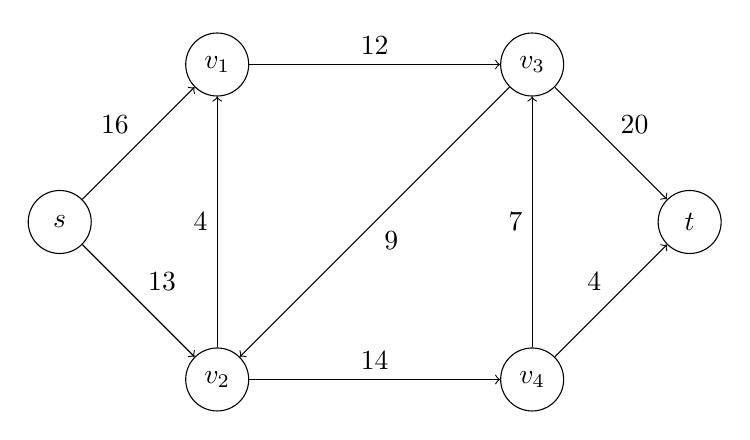
\begin{tikzpicture}[auto]
            \begin{scope}[every node/.style={circle,draw=black,minimum size=8mm}]
                \node (s) at (-4,0) {$s$};
                \node (v1) at (-2,2) {$v_1$};
                \node (v2) at (-2,-2) {$v_2$};
                \node (v3) at (2,2) {$v_3$};
                \node (v4) at (2,-2) {$v_4$};
                \node (t) at (4,0) {$t$};
            \end{scope}
            \draw (s) edge [->] node{16} (v1);
            \draw (v1) edge [->] node{12} (v3);
            \draw (v3) edge [->] node{20} (t);
            \draw (s) edge [->] node{13} (v2);
            \draw (v2) edge [->] node{14} (v4);
            \draw (v4) edge [->] node{4} (t);
            \draw (v2) edge [->] node{4} (v1);
            \draw (v3) edge [->] node{9} (v2);
            \draw (v4) edge [->] node{7} (v3);
        \end{tikzpicture}\\
        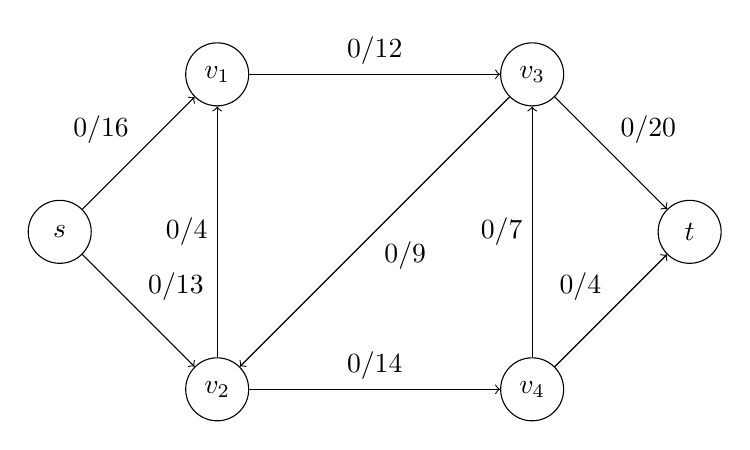
\begin{tikzpicture}[auto]
            \begin{scope}[every node/.style={circle,draw=black,minimum size=8mm}]
                \node (s) at (-4,0) {$s$};
                \node (v1) at (-2,2) {$v_1$};
                \node (v2) at (-2,-2) {$v_2$};
                \node (v3) at (2,2) {$v_3$};
                \node (v4) at (2,-2) {$v_4$};
                \node (t) at (4,0) {$t$};
            \end{scope}
            \draw (s) edge [->] node{0/16} (v1);
            \draw (v1) edge [->] node{0/12} (v3);
            \draw (v3) edge [->] node{0/20} (t);
            \draw (s) edge [->] node{0/13} (v2);
            \draw (v2) edge [->] node{0/14} (v4);
            \draw (v4) edge [->] node{0/4} (t);
            \draw (v2) edge [->] node{0/4} (v1);
            \draw (v3) edge [->] node{0/9} (v2);
            \draw (v4) edge [->] node{0/7} (v3);
        \end{tikzpicture}\\
        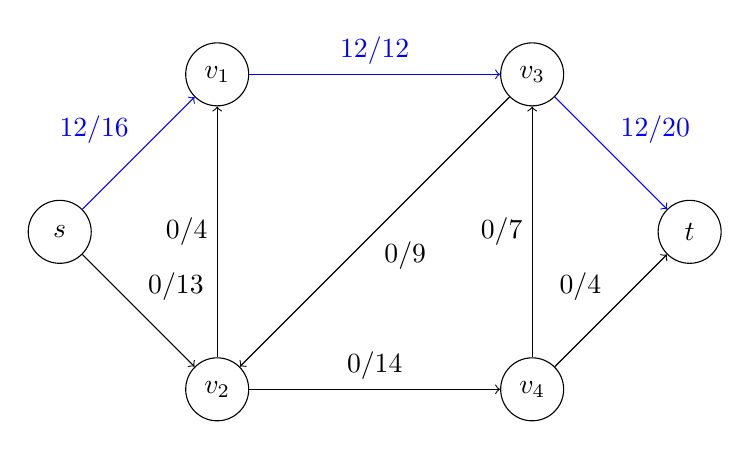
\begin{tikzpicture}[auto]
            \begin{scope}[every node/.style={circle,draw=black,minimum size=8mm}]
                \node (s) at (-4,0) {$s$};
                \node (v1) at (-2,2) {$v_1$};
                \node (v2) at (-2,-2) {$v_2$};
                \node (v3) at (2,2) {$v_3$};
                \node (v4) at (2,-2) {$v_4$};
                \node (t) at (4,0) {$t$};
            \end{scope}
            \draw (s) edge [->, blue] node{12/16} (v1);
            \draw (v1) edge [->, blue] node{12/12} (v3);
            \draw (v3) edge [->, blue] node{12/20} (t);
            \draw (s) edge [->] node{0/13} (v2);
            \draw (v2) edge [->] node{0/14} (v4);
            \draw (v4) edge [->] node{0/4} (t);
            \draw (v2) edge [->] node{0/4} (v1);
            \draw (v3) edge [->] node{0/9} (v2);
            \draw (v4) edge [->] node{0/7} (v3);
        \end{tikzpicture}\\
        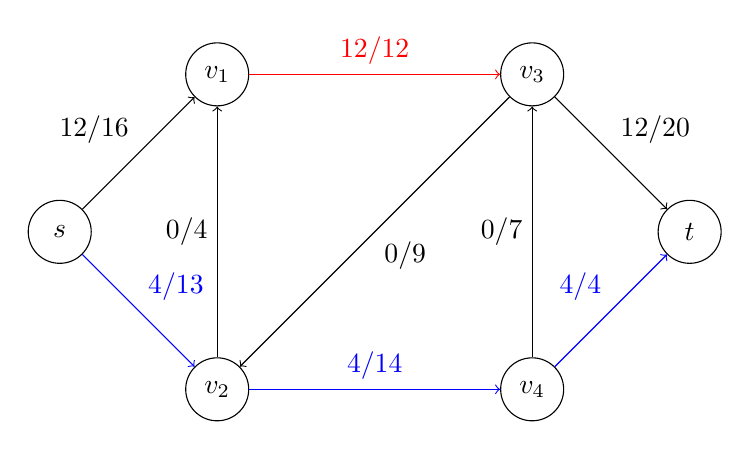
\begin{tikzpicture}[auto]
            \begin{scope}[every node/.style={circle,draw=black,minimum size=8mm}]
                \node (s) at (-4,0) {$s$};
                \node (v1) at (-2,2) {$v_1$};
                \node (v2) at (-2,-2) {$v_2$};
                \node (v3) at (2,2) {$v_3$};
                \node (v4) at (2,-2) {$v_4$};
                \node (t) at (4,0) {$t$};
            \end{scope}
            \draw (s) edge [->] node{12/16} (v1);
            \draw (v1) edge [->, red] node{12/12} (v3);
            \draw (v3) edge [->] node{12/20} (t);
            \draw (s) edge [->, blue] node{4/13} (v2);
            \draw (v2) edge [->, blue] node{4/14} (v4);
            \draw (v4) edge [->, blue] node{4/4} (t);
            \draw (v2) edge [->] node{0/4} (v1);
            \draw (v3) edge [->] node{0/9} (v2);
            \draw (v4) edge [->] node{0/7} (v3);
        \end{tikzpicture}\\
        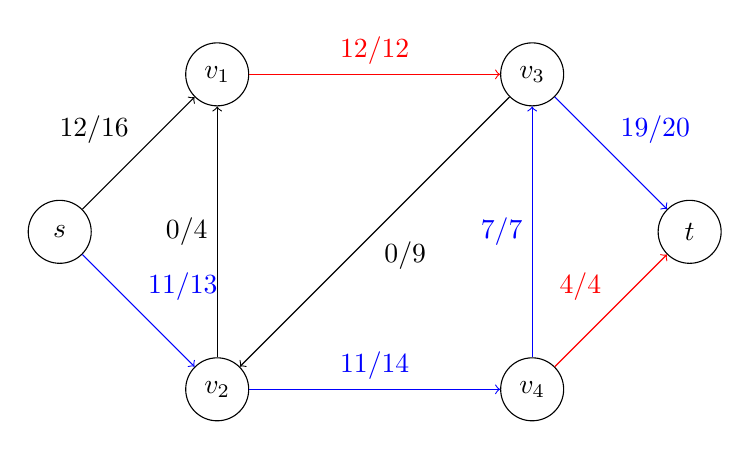
\begin{tikzpicture}[auto]
            \begin{scope}[every node/.style={circle,draw=black,minimum size=8mm}]
                \node (s) at (-4,0) {$s$};
                \node (v1) at (-2,2) {$v_1$};
                \node (v2) at (-2,-2) {$v_2$};
                \node (v3) at (2,2) {$v_3$};
                \node (v4) at (2,-2) {$v_4$};
                \node (t) at (4,0) {$t$};
            \end{scope}
            \draw (s) edge [->] node{12/16} (v1);
            \draw (v1) edge [->, red] node{12/12} (v3);
            \draw (v3) edge [->, blue] node{19/20} (t);
            \draw (s) edge [->, blue] node{11/13} (v2);
            \draw (v2) edge [->, blue] node{11/14} (v4);
            \draw (v4) edge [->, red] node{4/4} (t);
            \draw (v2) edge [->] node{0/4} (v1);
            \draw (v3) edge [->] node{0/9} (v2);
            \draw (v4) edge [->, blue] node{7/7} (v3);
        \end{tikzpicture}\\
        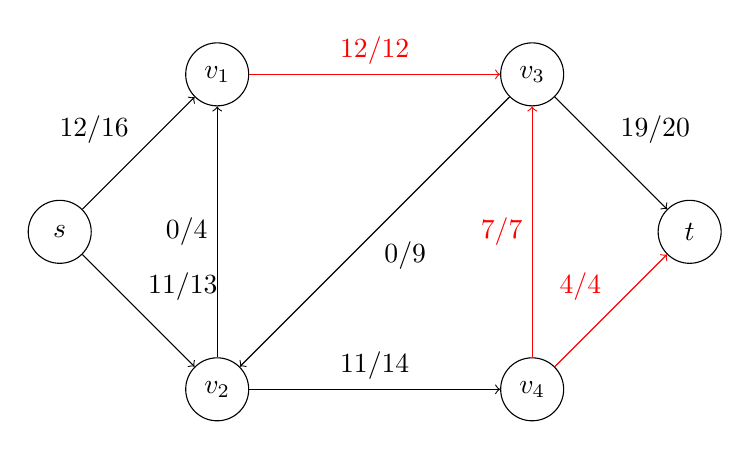
\begin{tikzpicture}[auto]
            \begin{scope}[every node/.style={circle,draw=black,minimum size=8mm}]
                \node (s) at (-4,0) {$s$};
                \node (v1) at (-2,2) {$v_1$};
                \node (v2) at (-2,-2) {$v_2$};
                \node (v3) at (2,2) {$v_3$};
                \node (v4) at (2,-2) {$v_4$};
                \node (t) at (4,0) {$t$};
            \end{scope}
            \draw (s) edge [->] node{12/16} (v1);
            \draw (v1) edge [->, red] node{12/12} (v3);
            \draw (v3) edge [->] node{19/20} (t);
            \draw (s) edge [->] node{11/13} (v2);
            \draw (v2) edge [->] node{11/14} (v4);
            \draw (v4) edge [->, red] node{4/4} (t);
            \draw (v2) edge [->] node{0/4} (v1);
            \draw (v3) edge [->] node{0/9} (v2);
            \draw (v4) edge [->, red] node{7/7} (v3);
        \end{tikzpicture}
    \end{center}
    No Augmenting path $P$ where $c_f(P)>0\Rightarrow$ Maximum flow $f=12+11=23$.
\section{26.3-1} Run the Ford-Fulkerson algorithm on the flow network in Figure 26.8(b) and show the residual network after each flow augmentation. Number the vertices in $L$ top to bottom from $1$ to $5$ and in $R$ top to bottom from $6$ to $9$. For each iteration, pick the augmenting path that is lexicographically smallest.\\
\textcolor{blue}{Answer:}
First, construct $G'$ from Figure 26.8(b)
    \begin{center}
        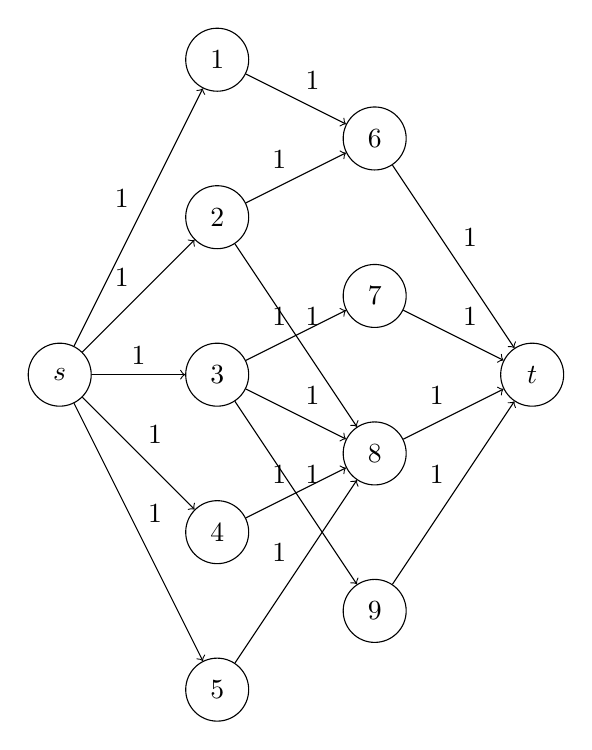
\begin{tikzpicture}[auto]
            \begin{scope}[every node/.style={circle,draw=black,minimum size=8mm}]
                \node (s) at (-4,0) {$s$};
                \node (v1) at (-2,4) {$1$};
                \node (v2) at (-2,2) {$2$};
                \node (v3) at (-2,0) {$3$};
                \node (v4) at (-2,-2) {$4$};
                \node (v5) at (-2,-4) {$5$};
                \node (v6) at (0,3) {$6$};
                \node (v7) at (0,1) {$7$};
                \node (v8) at (0,-1) {$8$};
                \node (v9) at (0,-3) {$9$};
                \node (t) at (2,0) {$t$};
            \end{scope}
            \draw (s) edge [->] node{1} (v1);
            \draw (s) edge [->] node{1} (v2);
            \draw (s) edge [->] node{1} (v3);
            \draw (s) edge [->] node{1} (v4);
            \draw (s) edge [->] node{1} (v5);
            \draw (v1) edge [->] node{1} (v6);
            \draw (v2) edge [->] node{1} (v6);
            \draw (v2) edge [->] node{1} (v8);
            \draw (v3) edge [->] node{1} (v7);
            \draw (v3) edge [->] node{1} (v8);
            \draw (v3) edge [->] node{1} (v9);
            \draw (v4) edge [->] node{1} (v8);
            \draw (v5) edge [->] node{1} (v8);
            \draw (v6) edge [->] node{1} (t);
            \draw (v7) edge [->] node{1} (t);
            \draw (v8) edge [->] node{1} (t);
            \draw (v9) edge [->] node{1} (t);
        \end{tikzpicture}\\
        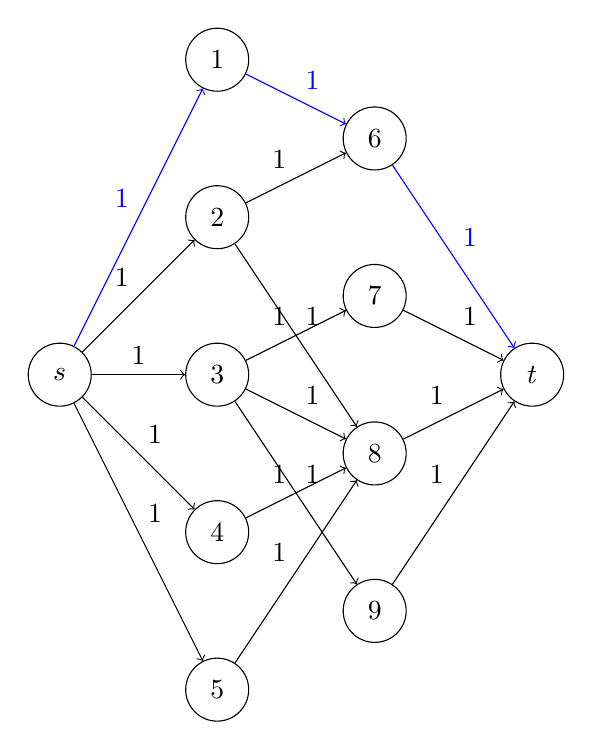
\begin{tikzpicture}[auto]
            \begin{scope}[every node/.style={circle,draw=black,minimum size=8mm}]
                \node (s) at (-4,0) {$s$};
                \node (v1) at (-2,4) {$1$};
                \node (v2) at (-2,2) {$2$};
                \node (v3) at (-2,0) {$3$};
                \node (v4) at (-2,-2) {$4$};
                \node (v5) at (-2,-4) {$5$};
                \node (v6) at (0,3) {$6$};
                \node (v7) at (0,1) {$7$};
                \node (v8) at (0,-1) {$8$};
                \node (v9) at (0,-3) {$9$};
                \node (t) at (2,0) {$t$};
            \end{scope}
            \draw (s) edge [->, blue] node{1} (v1);
            \draw (s) edge [->] node{1} (v2);
            \draw (s) edge [->] node{1} (v3);
            \draw (s) edge [->] node{1} (v4);
            \draw (s) edge [->] node{1} (v5);
            \draw (v1) edge [->, blue] node{1} (v6);
            \draw (v2) edge [->] node{1} (v6);
            \draw (v2) edge [->] node{1} (v8);
            \draw (v3) edge [->] node{1} (v7);
            \draw (v3) edge [->] node{1} (v8);
            \draw (v3) edge [->] node{1} (v9);
            \draw (v4) edge [->] node{1} (v8);
            \draw (v5) edge [->] node{1} (v8);
            \draw (v6) edge [->, blue] node{1} (t);
            \draw (v7) edge [->] node{1} (t);
            \draw (v8) edge [->] node{1} (t);
            \draw (v9) edge [->] node{1} (t);
        \end{tikzpicture}\\
        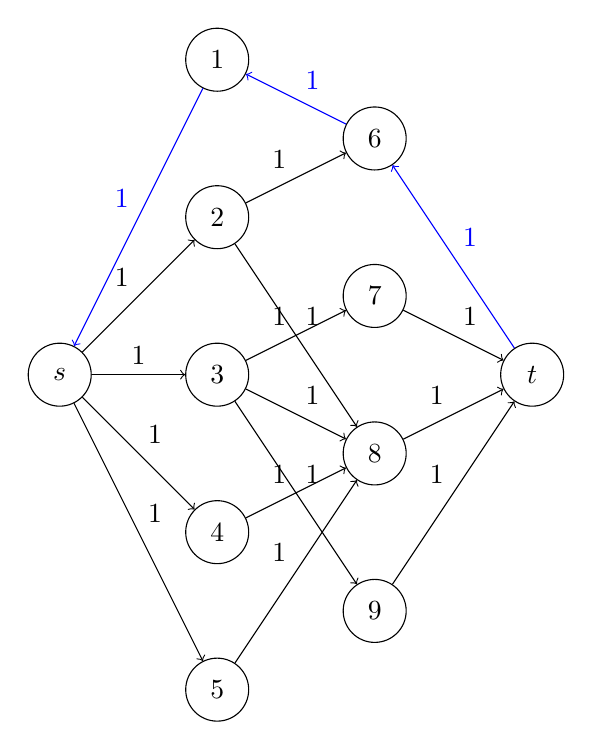
\begin{tikzpicture}[auto]
            \begin{scope}[every node/.style={circle,draw=black,minimum size=8mm}]
                \node (s) at (-4,0) {$s$};
                \node (v1) at (-2,4) {$1$};
                \node (v2) at (-2,2) {$2$};
                \node (v3) at (-2,0) {$3$};
                \node (v4) at (-2,-2) {$4$};
                \node (v5) at (-2,-4) {$5$};
                \node (v6) at (0,3) {$6$};
                \node (v7) at (0,1) {$7$};
                \node (v8) at (0,-1) {$8$};
                \node (v9) at (0,-3) {$9$};
                \node (t) at (2,0) {$t$};
            \end{scope}
            \draw (s) edge [<-, blue] node{1} (v1);
            \draw (s) edge [->] node{1} (v2);
            \draw (s) edge [->] node{1} (v3);
            \draw (s) edge [->] node{1} (v4);
            \draw (s) edge [->] node{1} (v5);
            \draw (v1) edge [<-, blue] node{1} (v6);
            \draw (v2) edge [->] node{1} (v6);
            \draw (v2) edge [->] node{1} (v8);
            \draw (v3) edge [->] node{1} (v7);
            \draw (v3) edge [->] node{1} (v8);
            \draw (v3) edge [->] node{1} (v9);
            \draw (v4) edge [->] node{1} (v8);
            \draw (v5) edge [->] node{1} (v8);
            \draw (v6) edge [<-, blue] node{1} (t);
            \draw (v7) edge [->] node{1} (t);
            \draw (v8) edge [->] node{1} (t);
            \draw (v9) edge [->] node{1} (t);
        \end{tikzpicture}\\
        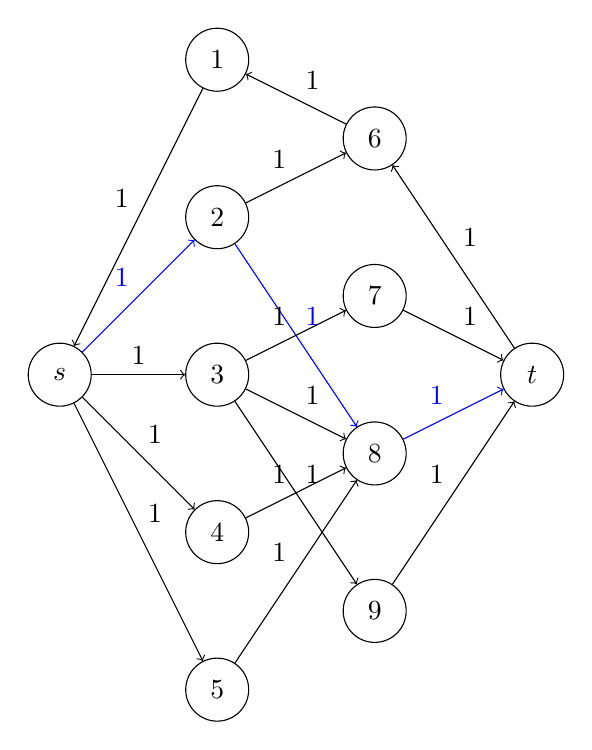
\begin{tikzpicture}[auto]
            \begin{scope}[every node/.style={circle,draw=black,minimum size=8mm}]
                \node (s) at (-4,0) {$s$};
                \node (v1) at (-2,4) {$1$};
                \node (v2) at (-2,2) {$2$};
                \node (v3) at (-2,0) {$3$};
                \node (v4) at (-2,-2) {$4$};
                \node (v5) at (-2,-4) {$5$};
                \node (v6) at (0,3) {$6$};
                \node (v7) at (0,1) {$7$};
                \node (v8) at (0,-1) {$8$};
                \node (v9) at (0,-3) {$9$};
                \node (t) at (2,0) {$t$};
            \end{scope}
            \draw (s) edge [<-] node{1} (v1);
            \draw (s) edge [->, blue] node{1} (v2);
            \draw (s) edge [->] node{1} (v3);
            \draw (s) edge [->] node{1} (v4);
            \draw (s) edge [->] node{1} (v5);
            \draw (v1) edge [<-] node{1} (v6);
            \draw (v2) edge [->] node{1} (v6);
            \draw (v2) edge [->, blue] node{1} (v8);
            \draw (v3) edge [->] node{1} (v7);
            \draw (v3) edge [->] node{1} (v8);
            \draw (v3) edge [->] node{1} (v9);
            \draw (v4) edge [->] node{1} (v8);
            \draw (v5) edge [->] node{1} (v8);
            \draw (v6) edge [<-] node{1} (t);
            \draw (v7) edge [->] node{1} (t);
            \draw (v8) edge [->, blue] node{1} (t);
            \draw (v9) edge [->] node{1} (t);
        \end{tikzpicture}\\
        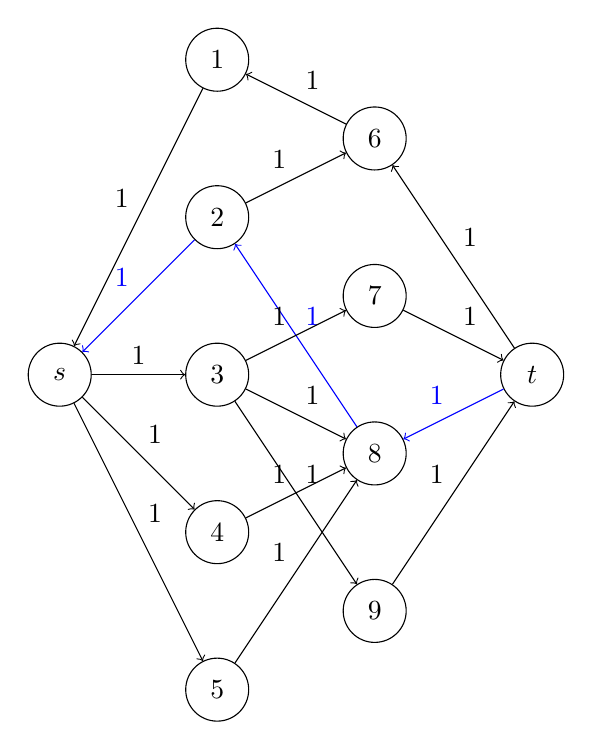
\begin{tikzpicture}[auto]
            \begin{scope}[every node/.style={circle,draw=black,minimum size=8mm}]
                \node (s) at (-4,0) {$s$};
                \node (v1) at (-2,4) {$1$};
                \node (v2) at (-2,2) {$2$};
                \node (v3) at (-2,0) {$3$};
                \node (v4) at (-2,-2) {$4$};
                \node (v5) at (-2,-4) {$5$};
                \node (v6) at (0,3) {$6$};
                \node (v7) at (0,1) {$7$};
                \node (v8) at (0,-1) {$8$};
                \node (v9) at (0,-3) {$9$};
                \node (t) at (2,0) {$t$};
            \end{scope}
            \draw (s) edge [<-] node{1} (v1);
            \draw (s) edge [<-, blue] node{1} (v2);
            \draw (s) edge [->] node{1} (v3);
            \draw (s) edge [->] node{1} (v4);
            \draw (s) edge [->] node{1} (v5);
            \draw (v1) edge [<-] node{1} (v6);
            \draw (v2) edge [->] node{1} (v6);
            \draw (v2) edge [<-, blue] node{1} (v8);
            \draw (v3) edge [->] node{1} (v7);
            \draw (v3) edge [->] node{1} (v8);
            \draw (v3) edge [->] node{1} (v9);
            \draw (v4) edge [->] node{1} (v8);
            \draw (v5) edge [->] node{1} (v8);
            \draw (v6) edge [<-] node{1} (t);
            \draw (v7) edge [->] node{1} (t);
            \draw (v8) edge [<-, blue] node{1} (t);
            \draw (v9) edge [->] node{1} (t);
        \end{tikzpicture}\\
        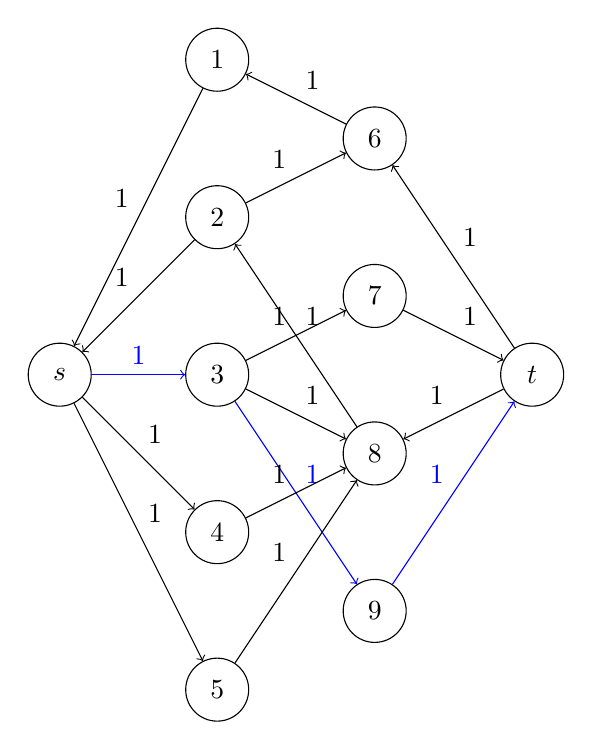
\begin{tikzpicture}[auto]
            \begin{scope}[every node/.style={circle,draw=black,minimum size=8mm}]
                \node (s) at (-4,0) {$s$};
                \node (v1) at (-2,4) {$1$};
                \node (v2) at (-2,2) {$2$};
                \node (v3) at (-2,0) {$3$};
                \node (v4) at (-2,-2) {$4$};
                \node (v5) at (-2,-4) {$5$};
                \node (v6) at (0,3) {$6$};
                \node (v7) at (0,1) {$7$};
                \node (v8) at (0,-1) {$8$};
                \node (v9) at (0,-3) {$9$};
                \node (t) at (2,0) {$t$};
            \end{scope}
            \draw (s) edge [<-] node{1} (v1);
            \draw (s) edge [<-] node{1} (v2);
            \draw (s) edge [->, blue] node{1} (v3);
            \draw (s) edge [->] node{1} (v4);
            \draw (s) edge [->] node{1} (v5);
            \draw (v1) edge [<-] node{1} (v6);
            \draw (v2) edge [->] node{1} (v6);
            \draw (v2) edge [<-] node{1} (v8);
            \draw (v3) edge [->] node{1} (v7);
            \draw (v3) edge [->] node{1} (v8);
            \draw (v3) edge [->, blue] node{1} (v9);
            \draw (v4) edge [->] node{1} (v8);
            \draw (v5) edge [->] node{1} (v8);
            \draw (v6) edge [<-] node{1} (t);
            \draw (v7) edge [->] node{1} (t);
            \draw (v8) edge [<-] node{1} (t);
            \draw (v9) edge [->, blue] node{1} (t);
        \end{tikzpicture}\\
        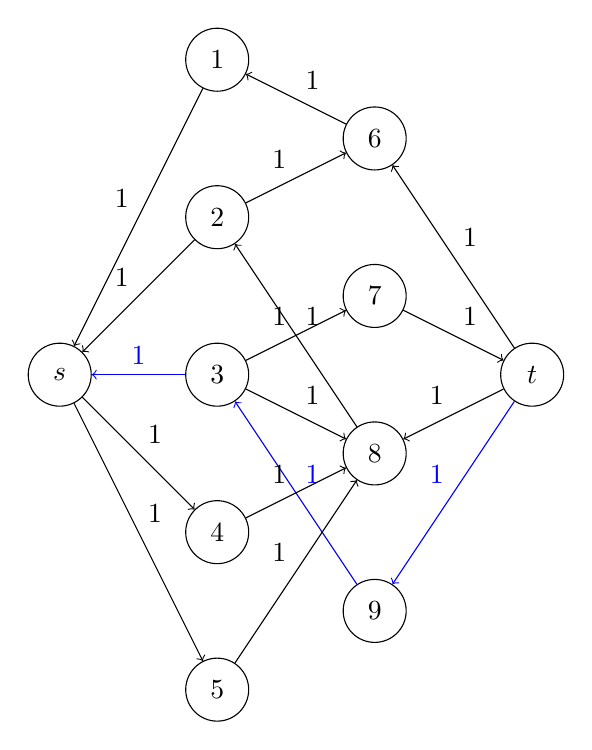
\begin{tikzpicture}[auto]
            \begin{scope}[every node/.style={circle,draw=black,minimum size=8mm}]
                \node (s) at (-4,0) {$s$};
                \node (v1) at (-2,4) {$1$};
                \node (v2) at (-2,2) {$2$};
                \node (v3) at (-2,0) {$3$};
                \node (v4) at (-2,-2) {$4$};
                \node (v5) at (-2,-4) {$5$};
                \node (v6) at (0,3) {$6$};
                \node (v7) at (0,1) {$7$};
                \node (v8) at (0,-1) {$8$};
                \node (v9) at (0,-3) {$9$};
                \node (t) at (2,0) {$t$};
            \end{scope}
            \draw (s) edge [<-] node{1} (v1);
            \draw (s) edge [<-] node{1} (v2);
            \draw (s) edge [<-, blue] node{1} (v3);
            \draw (s) edge [->] node{1} (v4);
            \draw (s) edge [->] node{1} (v5);
            \draw (v1) edge [<-] node{1} (v6);
            \draw (v2) edge [->] node{1} (v6);
            \draw (v2) edge [<-] node{1} (v8);
            \draw (v3) edge [->] node{1} (v7);
            \draw (v3) edge [->] node{1} (v8);
            \draw (v3) edge [<-, blue] node{1} (v9);
            \draw (v4) edge [->] node{1} (v8);
            \draw (v5) edge [->] node{1} (v8);
            \draw (v6) edge [<-] node{1} (t);
            \draw (v7) edge [->] node{1} (t);
            \draw (v8) edge [<-] node{1} (t);
            \draw (v9) edge [<-, blue] node{1} (t);
        \end{tikzpicture}\\
        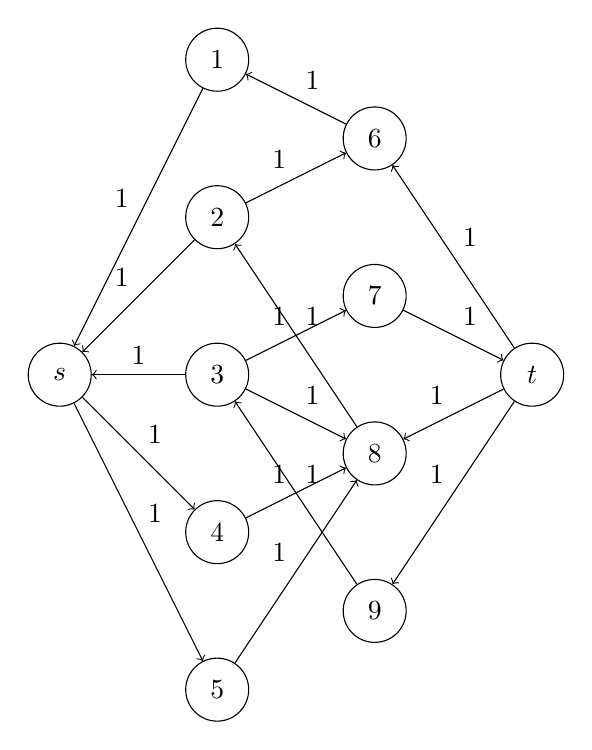
\begin{tikzpicture}[auto]
            \begin{scope}[every node/.style={circle,draw=black,minimum size=8mm}]
                \node (s) at (-4,0) {$s$};
                \node (v1) at (-2,4) {$1$};
                \node (v2) at (-2,2) {$2$};
                \node (v3) at (-2,0) {$3$};
                \node (v4) at (-2,-2) {$4$};
                \node (v5) at (-2,-4) {$5$};
                \node (v6) at (0,3) {$6$};
                \node (v7) at (0,1) {$7$};
                \node (v8) at (0,-1) {$8$};
                \node (v9) at (0,-3) {$9$};
                \node (t) at (2,0) {$t$};
            \end{scope}
            \draw (s) edge [<-] node{1} (v1);
            \draw (s) edge [<-] node{1} (v2);
            \draw (s) edge [<-] node{1} (v3);
            \draw (s) edge [->] node{1} (v4);
            \draw (s) edge [->] node{1} (v5);
            \draw (v1) edge [<-] node{1} (v6);
            \draw (v2) edge [->] node{1} (v6);
            \draw (v2) edge [<-] node{1} (v8);
            \draw (v3) edge [->] node{1} (v7);
            \draw (v3) edge [->] node{1} (v8);
            \draw (v3) edge [<-] node{1} (v9);
            \draw (v4) edge [->] node{1} (v8);
            \draw (v5) edge [->] node{1} (v8);
            \draw (v6) edge [<-] node{1} (t);
            \draw (v7) edge [->] node{1} (t);
            \draw (v8) edge [<-] node{1} (t);
            \draw (v9) edge [<-] node{1} (t);
        \end{tikzpicture}
    \end{center}
    There is no more path from $s$ to $t$ in the residual network $G_f$, we have done, the maximum flow is $3$.
\end{document}

